\documentclass[10pt,a4paper]{article}
\usepackage[T1]{fontenc}
\usepackage[utf8]{inputenc}
\usepackage{lmodern}
\usepackage[a4paper,left=38mm,right=38mm,top=34mm,bottom=38mm]{geometry}
\usepackage{amsmath,amssymb}
\usepackage{xcolor}
\usepackage{tikz}
\usetikzlibrary{arrows.meta,patterns}
\usepackage{float}
\usepackage[font=small,labelfont=bf,skip=6pt]{caption}
\usepackage{booktabs}
\usepackage{enumitem}
\usepackage[hidelinks]{hyperref}
\setlength{\parindent}{0pt}
\setlength{\parskip}{0.55em}
\setlength{\textfloatsep}{14pt}
\setlength{\intextsep}{14pt}

\definecolor{ink}{HTML}{1D2733}
\definecolor{inksoft}{HTML}{55606C}
\definecolor{gridc}{HTML}{BCC2BA}
\definecolor{chosen}{HTML}{24525F}
\definecolor{blockedc}{HTML}{C9CEC7}
\definecolor{hatch}{HTML}{8F978E}
\definecolor{candc}{HTML}{C27A12}
\definecolor{candtint}{HTML}{F6DFB6}
\definecolor{cand2c}{HTML}{6D55B3}
\definecolor{cand2tint}{HTML}{DDD5F3}
\definecolor{focus}{HTML}{2C7DA0}
\definecolor{focustint}{HTML}{CFE6EF}
\definecolor{bad}{HTML}{C0392B}
\definecolor{okc}{HTML}{3F7D4A}

\newcommand{\incode}{\textsf{\scriptsize\color{okc}[in code]}}
\newcommand{\proposed}{\textsf{\scriptsize\color{candc}[proposed]}}
\newcommand{\onmap}{\par\medskip\textsf{\small\bfseries\color{inksoft}On the map}\par}
\newcommand{\interms}{\par\medskip\textsf{\small\bfseries\color{inksoft}In .conditions}\par}
\newcommand{\code}[1]{\texttt{#1}}
\newcommand{\T}[1]{\ensuremath{\{#1\}}}
\newenvironment{algebra}{\begin{center}\begin{minipage}{0.92\linewidth}\small\setlength{\parskip}{0.2em}}{\end{minipage}\end{center}}
\newcommand{\cmt}[1]{{\color{inksoft}\textit{#1}}}

\title{\textsf{Conditions and the Map}\\[0.3em]\large SquarePlacement foundations, draft 1}
\date{14 November 2026}
\author{}

\begin{document}
\maketitle
\thispagestyle{empty}

The algorithm keeps two descriptions of one situation: the \emph{map} (cells that are free, chosen or blocked, and the pixels they cover) and the \emph{.conditions algebra} (each free cell's set of terms). This draft puts the two side by side for every notion, from a single condition up to a refutation. The n-ary step is left out.

Every map and every term below is computed from the code (\code{conditions.initial\_map} and \code{bruteforce.compute\_conditions}) by \code{docs/foundation/examples.py}. Statements are marked \incode{} when the code does this today and \proposed{} when it is a design step still to be made.

\paragraph{Legend.}
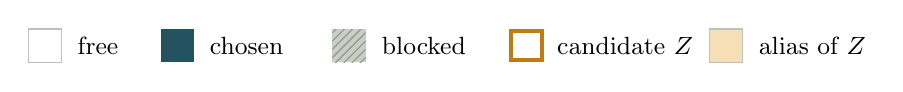
\begin{tikzpicture}[x=0.42cm,y=0.42cm,baseline=-3pt]
\fill[white] (0,0) rectangle (1,-1); \draw[gridc] (0,0) rectangle (1,-1); \node[anchor=west,font=\small] at (1.2,-0.5) {free};
\fill[chosen] (4,0) rectangle (5,-1); \node[anchor=west,font=\small] at (5.2,-0.5) {chosen};
\fill[blockedc] (9.2,0) rectangle (10.2,-1); \fill[pattern=north east lines,pattern color=hatch] (9.2,0) rectangle (10.2,-1); \node[anchor=west,font=\small] at (10.4,-0.5) {blocked};
\draw[candc,line width=1.4pt] (14.6,-0.07) rectangle (15.53,-0.93); \node[anchor=west,font=\small] at (15.7,-0.5) {candidate $Z$};
\fill[candtint] (20.6,0) rectangle (21.6,-1); \draw[gridc] (20.6,0) rectangle (21.6,-1); \node[anchor=west,font=\small] at (21.8,-0.5) {alias of $Z$};
\end{tikzpicture}


\begin{tikzpicture}[x=0.42cm,y=0.42cm,baseline=-3pt]
\draw[ink,line width=0.9pt] (0.5,-0.5) circle (0.3); \node[anchor=west,font=\small] at (1.2,-0.5) {term member};
\draw[-{Stealth[length=3.2pt]},ink,line width=0.8pt] (6.4,-0.5) -- (7.8,-0.5); \node[anchor=west,font=\small] at (8,-0.5) {link $a\to y$};
\draw[-{Stealth[length=3.2pt]},inksoft,densely dashed,line width=0.6pt] (11.6,-0.5) -- (13,-0.5); \node[anchor=west,font=\small] at (13.2,-0.5) {blocks};
\filldraw[fill=white,draw=ink,line width=0.7pt] (16.5,-0.5) circle (0.13); \node[anchor=west,font=\small] at (16.8,-0.5) {pixel};
\filldraw[fill=white,draw=bad,line width=0.9pt] (19.5,-0.5) circle (0.26); \draw[bad,line width=1pt] (19.33,-0.33) -- (19.67,-0.67) (19.33,-0.67) -- (19.67,-0.33); \node[anchor=west,font=\small] at (19.9,-0.5) {uncoverable pixel};
\end{tikzpicture}


\begin{tikzpicture}[x=0.42cm,y=0.42cm,baseline=-3pt]
\draw[bad,line width=1pt] (0.5,-0.5) circle (0.4); \node[anchor=west,font=\small] at (1.2,-0.5) {cells blocking each other};
\draw[focus,line width=0.9pt,rounded corners=1.5pt] (12,0) rectangle (13.4,-1); \node[anchor=west,font=\small] at (13.6,-0.5) {a 2$\times$2 block (outline)};
\end{tikzpicture}

%------------------------------------------------------------------
\section{What are .conditions?}

A cell $(r,c)$ is the position of one 2$\times$2 square; its square covers the pixels $(r..r{+}1,\ c..c{+}1)$. In the maps, cells are boxes and \textbf{pixels are the grid points}: a cell covers the four grid points at its corners. The four cells around a grid point form a \textbf{2$\times$2 block}; they are the only cells that can cover that pixel.

\onmap
\begin{figure}[H]\centering
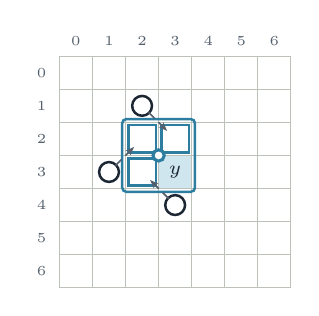
\begin{tikzpicture}[x=0.42cm,y=0.42cm,baseline=(current bounding box.north)]
\node[font=\tiny,text=inksoft] at (0.5,0.45) {0};
\node[font=\tiny,text=inksoft] at (1.5,0.45) {1};
\node[font=\tiny,text=inksoft] at (2.5,0.45) {2};
\node[font=\tiny,text=inksoft] at (3.5,0.45) {3};
\node[font=\tiny,text=inksoft] at (4.5,0.45) {4};
\node[font=\tiny,text=inksoft] at (5.5,0.45) {5};
\node[font=\tiny,text=inksoft] at (6.5,0.45) {6};
\node[font=\tiny,text=inksoft,anchor=east] at (-0.1,-0.5) {0};
\node[font=\tiny,text=inksoft,anchor=east] at (-0.1,-1.5) {1};
\node[font=\tiny,text=inksoft,anchor=east] at (-0.1,-2.5) {2};
\node[font=\tiny,text=inksoft,anchor=east] at (-0.1,-3.5) {3};
\node[font=\tiny,text=inksoft,anchor=east] at (-0.1,-4.5) {4};
\node[font=\tiny,text=inksoft,anchor=east] at (-0.1,-5.5) {5};
\node[font=\tiny,text=inksoft,anchor=east] at (-0.1,-6.5) {6};
\fill[focustint] (3,-3) rectangle (4,-4);
\draw[gridc,line width=0.3pt,step=1] (0,-7) grid (7,0);
\draw[ink,line width=0.9pt] (2.5,-1.5) circle (0.3);
\draw[focus,line width=0.8pt] (2.09,-2.09) rectangle (2.91,-2.91);
\draw[focus,line width=0.8pt] (3.09,-2.09) rectangle (3.91,-2.91);
\draw[ink,line width=0.9pt] (1.5,-3.5) circle (0.3);
\draw[focus,line width=0.8pt] (2.09,-3.09) rectangle (2.91,-3.91);
\draw[ink,line width=0.9pt] (3.5,-4.5) circle (0.3);
\draw[focus,line width=0.9pt,rounded corners=1.5pt] (1.9,-1.9) rectangle (4.1,-4.1);
\filldraw[fill=white,draw=focus,line width=1.1pt] (3,-3) circle (0.17);
\draw[-{Stealth[length=3.2pt]},inksoft,densely dashed,line width=0.6pt,shorten <=0.118cm,shorten >=0.143cm] (1.5,-3.5) -- (2.5,-2.5);
\draw[-{Stealth[length=3.2pt]},inksoft,densely dashed,line width=0.6pt,shorten <=0.118cm,shorten >=0.143cm] (2.5,-1.5) -- (3.5,-2.5);
\draw[-{Stealth[length=3.2pt]},inksoft,densely dashed,line width=0.6pt,shorten <=0.118cm,shorten >=0.143cm] (3.5,-4.5) -- (2.5,-3.5);
\node[font=\scriptsize\bfseries,text=ink] at (3.5,-3.5) {$y$};
\end{tikzpicture}
\caption{The block above-left of $y=(3,3)$ covers the marked pixel. Each of its three other corners gets one blocker, a cell diagonal to that corner (dashed arrows).}
\end{figure}
If the three other corners of a block around $y$ are blocked, only $y$ can still cover the block's pixel, so $y$ must be chosen. A corner is blocked by a chosen diagonal neighbour. Each corner gets one such blocker, and the blockers obey the rules a placement must obey anyway: no two are diagonal to each other, none sits in the block, and none is a diagonal neighbour of $y$ (it would block $y$ itself).

\interms
\begin{algebra}
$(3,3).\mathtt{forced\_by} \ni \T{(1,2),\,(3,1),\,(4,3)}$\\
\cmt{read: } $\mathrm{chosen}(1,2)\wedge\mathrm{chosen}(3,1)\wedge\mathrm{chosen}(4,3)\Rightarrow\mathrm{chosen}(3,3)$
\end{algebra}
\code{y.forced\_by} is a set of \textbf{terms}. A term is a set of member ids; when all members are chosen, $y$ must be chosen. Logically each term is a Horn clause with only positive literals $\mathrm{chosen}(\cdot)$.

In the vacuum every interior cell has \textbf{76 terms}: four blocks around it, every admissible choice of blockers, a triple serving two blocks counted once. Terms with an off-board member are dropped, so cells near the edge have fewer.

A term names the \textbf{blockers}, never the corners. Which corner a member blocks, and which block the term came from, is not stored. This matters in sections 3 and 4.

%------------------------------------------------------------------
\section{Placing (choosing) a cell}

\onmap
\begin{figure}[H]\centering
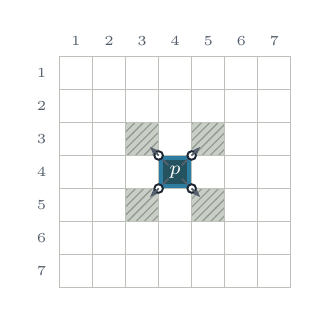
\begin{tikzpicture}[x=0.42cm,y=0.42cm,baseline=(current bounding box.north)]
\node[font=\tiny,text=inksoft] at (0.5,0.45) {1};
\node[font=\tiny,text=inksoft] at (1.5,0.45) {2};
\node[font=\tiny,text=inksoft] at (2.5,0.45) {3};
\node[font=\tiny,text=inksoft] at (3.5,0.45) {4};
\node[font=\tiny,text=inksoft] at (4.5,0.45) {5};
\node[font=\tiny,text=inksoft] at (5.5,0.45) {6};
\node[font=\tiny,text=inksoft] at (6.5,0.45) {7};
\node[font=\tiny,text=inksoft,anchor=east] at (-0.1,-0.5) {1};
\node[font=\tiny,text=inksoft,anchor=east] at (-0.1,-1.5) {2};
\node[font=\tiny,text=inksoft,anchor=east] at (-0.1,-2.5) {3};
\node[font=\tiny,text=inksoft,anchor=east] at (-0.1,-3.5) {4};
\node[font=\tiny,text=inksoft,anchor=east] at (-0.1,-4.5) {5};
\node[font=\tiny,text=inksoft,anchor=east] at (-0.1,-5.5) {6};
\node[font=\tiny,text=inksoft,anchor=east] at (-0.1,-6.5) {7};
\fill[blockedc] (2,-2) rectangle (3,-3);
\fill[pattern=north east lines,pattern color=hatch] (2,-2) rectangle (3,-3);
\fill[blockedc] (4,-2) rectangle (5,-3);
\fill[pattern=north east lines,pattern color=hatch] (4,-2) rectangle (5,-3);
\fill[chosen] (3,-3) rectangle (4,-4);
\fill[blockedc] (2,-4) rectangle (3,-5);
\fill[pattern=north east lines,pattern color=hatch] (2,-4) rectangle (3,-5);
\fill[blockedc] (4,-4) rectangle (5,-5);
\fill[pattern=north east lines,pattern color=hatch] (4,-4) rectangle (5,-5);
\draw[gridc,line width=0.3pt,step=1] (0,-7) grid (7,0);
\draw[focus,line width=1.4pt] (3.07,-3.07) rectangle (3.93,-3.93);
\filldraw[fill=white,draw=ink,line width=0.7pt] (3,-3) circle (0.13);
\filldraw[fill=white,draw=ink,line width=0.7pt] (4,-3) circle (0.13);
\filldraw[fill=white,draw=ink,line width=0.7pt] (3,-4) circle (0.13);
\filldraw[fill=white,draw=ink,line width=0.7pt] (4,-4) circle (0.13);
\draw[-{Stealth[length=3.2pt]},inksoft,densely dashed,line width=0.6pt,shorten <=0.118cm,shorten >=0.143cm] (3.5,-3.5) -- (2.5,-2.5);
\draw[-{Stealth[length=3.2pt]},inksoft,densely dashed,line width=0.6pt,shorten <=0.118cm,shorten >=0.143cm] (3.5,-3.5) -- (4.5,-2.5);
\draw[-{Stealth[length=3.2pt]},inksoft,densely dashed,line width=0.6pt,shorten <=0.118cm,shorten >=0.143cm] (3.5,-3.5) -- (2.5,-4.5);
\draw[-{Stealth[length=3.2pt]},inksoft,densely dashed,line width=0.6pt,shorten <=0.118cm,shorten >=0.143cm] (3.5,-3.5) -- (4.5,-4.5);
\node[font=\scriptsize\bfseries,text=white] at (3.5,-3.5) {$p$};
\end{tikzpicture}
\caption{$p=(4,4)$ chosen on a 9$\times$9 vacuum board. Its square covers the four marked pixels. Its four diagonal neighbours are blocked.}
\end{figure}
Choosing $p$ places its square. A direct neighbour may be chosen too: the two squares overlap along a whole edge and form a 3$\times$2 or 2$\times$3 shape. A diagonal neighbour may not: the two squares would overlap in a single pixel. So the moment $p$ is chosen, its four diagonal neighbours are blocked (section 3).

\interms
\begin{algebra}
$(2,5):\ \T{(1,3),\,(2,3),\,(4,4)} \;\longrightarrow\; \T{(1,3),\,(2,3)}$\\
\cmt{a member that is chosen drops out; the term survives, one shorter}
\end{algebra}
Wherever $p$ is a member, it drops out. On this board \textbf{228 terms} contain $(4,4)$; after the choice all of them are pairs. Chosen means \textbf{member satisfied}.

$p$'s own terms are cleared: a chosen cell has nothing left to be forced into. A term that loses its last member is true: its cell is forced (section 5). \incode{} \code{compute\_conditions}.

%------------------------------------------------------------------
\section{The four blocked cells of a placed cell}

\onmap
\begin{figure}[H]\centering
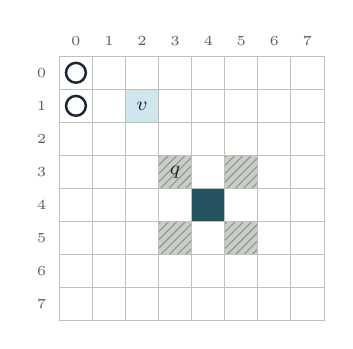
\begin{tikzpicture}[x=0.42cm,y=0.42cm,baseline=(current bounding box.north)]
\node[font=\tiny,text=inksoft] at (0.5,0.45) {0};
\node[font=\tiny,text=inksoft] at (1.5,0.45) {1};
\node[font=\tiny,text=inksoft] at (2.5,0.45) {2};
\node[font=\tiny,text=inksoft] at (3.5,0.45) {3};
\node[font=\tiny,text=inksoft] at (4.5,0.45) {4};
\node[font=\tiny,text=inksoft] at (5.5,0.45) {5};
\node[font=\tiny,text=inksoft] at (6.5,0.45) {6};
\node[font=\tiny,text=inksoft] at (7.5,0.45) {7};
\node[font=\tiny,text=inksoft,anchor=east] at (-0.1,-0.5) {0};
\node[font=\tiny,text=inksoft,anchor=east] at (-0.1,-1.5) {1};
\node[font=\tiny,text=inksoft,anchor=east] at (-0.1,-2.5) {2};
\node[font=\tiny,text=inksoft,anchor=east] at (-0.1,-3.5) {3};
\node[font=\tiny,text=inksoft,anchor=east] at (-0.1,-4.5) {4};
\node[font=\tiny,text=inksoft,anchor=east] at (-0.1,-5.5) {5};
\node[font=\tiny,text=inksoft,anchor=east] at (-0.1,-6.5) {6};
\node[font=\tiny,text=inksoft,anchor=east] at (-0.1,-7.5) {7};
\fill[focustint] (2,-1) rectangle (3,-2);
\fill[blockedc] (3,-3) rectangle (4,-4);
\fill[pattern=north east lines,pattern color=hatch] (3,-3) rectangle (4,-4);
\fill[blockedc] (5,-3) rectangle (6,-4);
\fill[pattern=north east lines,pattern color=hatch] (5,-3) rectangle (6,-4);
\fill[chosen] (4,-4) rectangle (5,-5);
\fill[blockedc] (3,-5) rectangle (4,-6);
\fill[pattern=north east lines,pattern color=hatch] (3,-5) rectangle (4,-6);
\fill[blockedc] (5,-5) rectangle (6,-6);
\fill[pattern=north east lines,pattern color=hatch] (5,-5) rectangle (6,-6);
\draw[gridc,line width=0.3pt,step=1] (0,-8) grid (8,0);
\draw[ink,line width=0.9pt] (0.5,-0.5) circle (0.3);
\draw[ink,line width=0.9pt] (0.5,-1.5) circle (0.3);
\node[font=\scriptsize\bfseries,text=ink] at (3.5,-3.5) {$q$};
\node[font=\scriptsize\bfseries,text=ink] at (2.5,-1.5) {$v$};
\end{tikzpicture}
\caption{After $p=(4,4)$: $q=(3,3)$ is one of its four blocked cells. The vacuum term $\T{(0,0),(1,0),(3,3)}$ of $v=(1,2)$ needed $q$ chosen. It is gone.}
\end{figure}
A blocked cell can never be chosen while $p$ stays chosen, and placements are not undone, so it is blocked for good. Its pixels can still be covered by other cells. Blocked says only that this cell's square will never be placed.

\interms
\begin{algebra}
$(1,2):\ \T{(0,0),\,(1,0),\,(3,3)} \;\longrightarrow\;$ {\color{bad}dropped}\\
\cmt{a member that is blocked can never be chosen: the term can never become true}
\end{algebra}
Wherever a blocked cell is a member, the term is \textbf{dead} and dropped. On this board \textbf{912 terms} have one of $p$'s four diagonals as a member. The blocked cells' own terms are cleared as well (380 terms, together with $p$'s). Blocked means \textbf{member impossible}.

Chosen and blocked are the two ways a member leaves a term: chosen, and the term shrinks; blocked, and the term dies.

After that, a blocked cell is never named in any term. As a member it has removed terms; as a corner it was never named at all (section 1). So a blocked cell has \textbf{no id in the algebra}. It exists only through what it did to the terms.

%------------------------------------------------------------------
\section[A blocked 2x2 block, and why it is impossible]{A blocked 2$\times$2 block, and why it is impossible}

\onmap
\begin{figure}[H]\centering
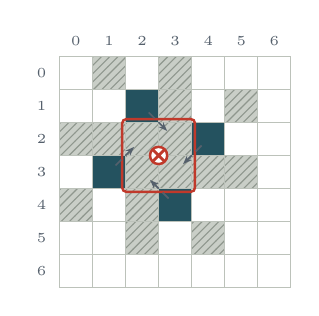
\begin{tikzpicture}[x=0.42cm,y=0.42cm,baseline=(current bounding box.north)]
\node[font=\tiny,text=inksoft] at (0.5,0.45) {0};
\node[font=\tiny,text=inksoft] at (1.5,0.45) {1};
\node[font=\tiny,text=inksoft] at (2.5,0.45) {2};
\node[font=\tiny,text=inksoft] at (3.5,0.45) {3};
\node[font=\tiny,text=inksoft] at (4.5,0.45) {4};
\node[font=\tiny,text=inksoft] at (5.5,0.45) {5};
\node[font=\tiny,text=inksoft] at (6.5,0.45) {6};
\node[font=\tiny,text=inksoft,anchor=east] at (-0.1,-0.5) {0};
\node[font=\tiny,text=inksoft,anchor=east] at (-0.1,-1.5) {1};
\node[font=\tiny,text=inksoft,anchor=east] at (-0.1,-2.5) {2};
\node[font=\tiny,text=inksoft,anchor=east] at (-0.1,-3.5) {3};
\node[font=\tiny,text=inksoft,anchor=east] at (-0.1,-4.5) {4};
\node[font=\tiny,text=inksoft,anchor=east] at (-0.1,-5.5) {5};
\node[font=\tiny,text=inksoft,anchor=east] at (-0.1,-6.5) {6};
\fill[blockedc] (1,0) rectangle (2,-1);
\fill[pattern=north east lines,pattern color=hatch] (1,0) rectangle (2,-1);
\fill[blockedc] (3,0) rectangle (4,-1);
\fill[pattern=north east lines,pattern color=hatch] (3,0) rectangle (4,-1);
\fill[chosen] (2,-1) rectangle (3,-2);
\fill[blockedc] (3,-1) rectangle (4,-2);
\fill[pattern=north east lines,pattern color=hatch] (3,-1) rectangle (4,-2);
\fill[blockedc] (5,-1) rectangle (6,-2);
\fill[pattern=north east lines,pattern color=hatch] (5,-1) rectangle (6,-2);
\fill[blockedc] (0,-2) rectangle (1,-3);
\fill[pattern=north east lines,pattern color=hatch] (0,-2) rectangle (1,-3);
\fill[blockedc] (1,-2) rectangle (2,-3);
\fill[pattern=north east lines,pattern color=hatch] (1,-2) rectangle (2,-3);
\fill[blockedc] (2,-2) rectangle (3,-3);
\fill[pattern=north east lines,pattern color=hatch] (2,-2) rectangle (3,-3);
\fill[blockedc] (3,-2) rectangle (4,-3);
\fill[pattern=north east lines,pattern color=hatch] (3,-2) rectangle (4,-3);
\fill[chosen] (4,-2) rectangle (5,-3);
\fill[chosen] (1,-3) rectangle (2,-4);
\fill[blockedc] (2,-3) rectangle (3,-4);
\fill[pattern=north east lines,pattern color=hatch] (2,-3) rectangle (3,-4);
\fill[blockedc] (3,-3) rectangle (4,-4);
\fill[pattern=north east lines,pattern color=hatch] (3,-3) rectangle (4,-4);
\fill[blockedc] (4,-3) rectangle (5,-4);
\fill[pattern=north east lines,pattern color=hatch] (4,-3) rectangle (5,-4);
\fill[blockedc] (5,-3) rectangle (6,-4);
\fill[pattern=north east lines,pattern color=hatch] (5,-3) rectangle (6,-4);
\fill[blockedc] (0,-4) rectangle (1,-5);
\fill[pattern=north east lines,pattern color=hatch] (0,-4) rectangle (1,-5);
\fill[blockedc] (2,-4) rectangle (3,-5);
\fill[pattern=north east lines,pattern color=hatch] (2,-4) rectangle (3,-5);
\fill[chosen] (3,-4) rectangle (4,-5);
\fill[blockedc] (2,-5) rectangle (3,-6);
\fill[pattern=north east lines,pattern color=hatch] (2,-5) rectangle (3,-6);
\fill[blockedc] (4,-5) rectangle (5,-6);
\fill[pattern=north east lines,pattern color=hatch] (4,-5) rectangle (5,-6);
\draw[gridc,line width=0.3pt,step=1] (0,-7) grid (7,0);
\draw[bad,line width=0.9pt,rounded corners=1.5pt] (1.9,-1.9) rectangle (4.1,-4.1);
\filldraw[fill=white,draw=bad,line width=0.9pt] (3,-3) circle (0.26);
\draw[bad,line width=1pt] (2.83,-2.83) -- (3.17,-3.17) (2.83,-3.17) -- (3.17,-2.83);
\draw[-{Stealth[length=3.2pt]},inksoft,densely dashed,line width=0.6pt,shorten <=0.118cm,shorten >=0.143cm] (1.5,-3.5) -- (2.5,-2.5);
\draw[-{Stealth[length=3.2pt]},inksoft,densely dashed,line width=0.6pt,shorten <=0.118cm,shorten >=0.143cm] (2.5,-1.5) -- (3.5,-2.5);
\draw[-{Stealth[length=3.2pt]},inksoft,densely dashed,line width=0.6pt,shorten <=0.118cm,shorten >=0.143cm] (3.5,-4.5) -- (2.5,-3.5);
\draw[-{Stealth[length=3.2pt]},inksoft,densely dashed,line width=0.6pt,shorten <=0.118cm,shorten >=0.143cm] (4.5,-2.5) -- (3.5,-3.5);
\end{tikzpicture}\hspace{1.2cm}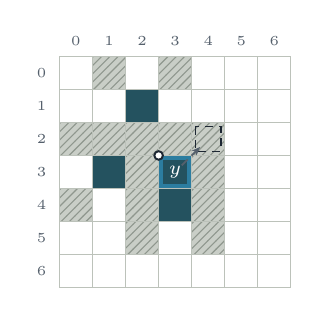
\begin{tikzpicture}[x=0.42cm,y=0.42cm,baseline=(current bounding box.north)]
\node[font=\tiny,text=inksoft] at (0.5,0.45) {0};
\node[font=\tiny,text=inksoft] at (1.5,0.45) {1};
\node[font=\tiny,text=inksoft] at (2.5,0.45) {2};
\node[font=\tiny,text=inksoft] at (3.5,0.45) {3};
\node[font=\tiny,text=inksoft] at (4.5,0.45) {4};
\node[font=\tiny,text=inksoft] at (5.5,0.45) {5};
\node[font=\tiny,text=inksoft] at (6.5,0.45) {6};
\node[font=\tiny,text=inksoft,anchor=east] at (-0.1,-0.5) {0};
\node[font=\tiny,text=inksoft,anchor=east] at (-0.1,-1.5) {1};
\node[font=\tiny,text=inksoft,anchor=east] at (-0.1,-2.5) {2};
\node[font=\tiny,text=inksoft,anchor=east] at (-0.1,-3.5) {3};
\node[font=\tiny,text=inksoft,anchor=east] at (-0.1,-4.5) {4};
\node[font=\tiny,text=inksoft,anchor=east] at (-0.1,-5.5) {5};
\node[font=\tiny,text=inksoft,anchor=east] at (-0.1,-6.5) {6};
\fill[blockedc] (1,0) rectangle (2,-1);
\fill[pattern=north east lines,pattern color=hatch] (1,0) rectangle (2,-1);
\fill[blockedc] (3,0) rectangle (4,-1);
\fill[pattern=north east lines,pattern color=hatch] (3,0) rectangle (4,-1);
\fill[chosen] (2,-1) rectangle (3,-2);
\fill[blockedc] (0,-2) rectangle (1,-3);
\fill[pattern=north east lines,pattern color=hatch] (0,-2) rectangle (1,-3);
\fill[blockedc] (1,-2) rectangle (2,-3);
\fill[pattern=north east lines,pattern color=hatch] (1,-2) rectangle (2,-3);
\fill[blockedc] (2,-2) rectangle (3,-3);
\fill[pattern=north east lines,pattern color=hatch] (2,-2) rectangle (3,-3);
\fill[blockedc] (3,-2) rectangle (4,-3);
\fill[pattern=north east lines,pattern color=hatch] (3,-2) rectangle (4,-3);
\fill[blockedc] (4,-2) rectangle (5,-3);
\fill[pattern=north east lines,pattern color=hatch] (4,-2) rectangle (5,-3);
\fill[chosen] (1,-3) rectangle (2,-4);
\fill[blockedc] (2,-3) rectangle (3,-4);
\fill[pattern=north east lines,pattern color=hatch] (2,-3) rectangle (3,-4);
\fill[chosen] (3,-3) rectangle (4,-4);
\fill[blockedc] (4,-3) rectangle (5,-4);
\fill[pattern=north east lines,pattern color=hatch] (4,-3) rectangle (5,-4);
\fill[blockedc] (0,-4) rectangle (1,-5);
\fill[pattern=north east lines,pattern color=hatch] (0,-4) rectangle (1,-5);
\fill[blockedc] (2,-4) rectangle (3,-5);
\fill[pattern=north east lines,pattern color=hatch] (2,-4) rectangle (3,-5);
\fill[chosen] (3,-4) rectangle (4,-5);
\fill[blockedc] (4,-4) rectangle (5,-5);
\fill[pattern=north east lines,pattern color=hatch] (4,-4) rectangle (5,-5);
\fill[blockedc] (2,-5) rectangle (3,-6);
\fill[pattern=north east lines,pattern color=hatch] (2,-5) rectangle (3,-6);
\fill[blockedc] (4,-5) rectangle (5,-6);
\fill[pattern=north east lines,pattern color=hatch] (4,-5) rectangle (5,-6);
\draw[gridc,line width=0.3pt,step=1] (0,-7) grid (7,0);
\draw[ink,densely dashed,line width=0.6pt] (4.12,-2.12) rectangle (4.88,-2.88);
\draw[focus,line width=1.4pt] (3.07,-3.07) rectangle (3.93,-3.93);
\filldraw[fill=white,draw=ink,line width=0.7pt] (3,-3) circle (0.13);
\draw[-{Stealth[length=3.2pt]},inksoft,densely dashed,line width=0.6pt,shorten <=0.118cm,shorten >=0.143cm] (3.5,-3.5) -- (4.5,-2.5);
\node[font=\scriptsize\bfseries,text=white] at (3.5,-3.5) {$y$};
\end{tikzpicture}
\caption{Left, hypothetical: the pinwheel $(3,1),(1,2),(2,4),(4,3)$ blocks all four cells around pixel $(3,3)$; no cell can cover it. Right, what actually happens: after three of the blockers, $(3,3)$ is a seat and is chosen (section 5), which blocks the fourth blocker $(2,4)$.}
\end{figure}
If all four cells of a block are blocked, the block's pixel can never be covered: a hole one pixel in size, the 1$\times$1 defect. The tiling can never be completed there, so this state must never be reached.

Legal play does not walk into it: once three corners are blocked, the fourth is a seat and gets chosen, and that blocks the fourth blocker. The seat rule exists to avoid the hole.

\interms
There is \textbf{no term} for this outcome today. A term always ends in a cell to choose; a hole has no cell. When a forced cell gets blocked, \code{compute\_conditions} clears that cell's terms, including the one that had just become true: the evidence is dropped.
\begin{algebra}
\cmt{defect term of the block around pixel (3,3):}\\
$\T{(3,1),\,(1,2),\,(4,3),\,(2,4)} \;\longrightarrow\; \bot$\\
\cmt{one blocker per corner, no two diagonal to each other}
\end{algebra}
\proposed{} The \textbf{defect term} $\T{m_1,m_2,m_3,m_4}\to\bot$ describes the hole in the language of terms: when all four members are chosen, the state is impossible. In the vacuum each block has \textbf{49} of them. It belongs to the block (the pixel), not to a cell.

It is the other half of a seat term. If $\T{m_1,m_2,m_3}\to y$ holds and $m_4$ is a cell that blocks $y$, then $\T{m_1,m_2,m_3,m_4}\to\bot$: choosing $m_4$ would block the cell the seat needs.

%------------------------------------------------------------------
\section{Seat rule and forcing, versus collapse and links}

The same fact twice: on the map, a seat forces a cell at the moment its third corner is blocked. In the terms, the condition collapses one member at a time, and its last-but-one stage, the single, is a link: the seat one placement in advance.

\begin{figure}[H]\centering
\begin{tabular}{@{}cccc@{}}
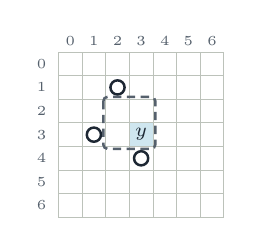
\begin{tikzpicture}[x=0.3cm,y=0.3cm,baseline=(current bounding box.north)]
\node[font=\tiny,text=inksoft] at (0.5,0.45) {0};
\node[font=\tiny,text=inksoft] at (1.5,0.45) {1};
\node[font=\tiny,text=inksoft] at (2.5,0.45) {2};
\node[font=\tiny,text=inksoft] at (3.5,0.45) {3};
\node[font=\tiny,text=inksoft] at (4.5,0.45) {4};
\node[font=\tiny,text=inksoft] at (5.5,0.45) {5};
\node[font=\tiny,text=inksoft] at (6.5,0.45) {6};
\node[font=\tiny,text=inksoft,anchor=east] at (-0.1,-0.5) {0};
\node[font=\tiny,text=inksoft,anchor=east] at (-0.1,-1.5) {1};
\node[font=\tiny,text=inksoft,anchor=east] at (-0.1,-2.5) {2};
\node[font=\tiny,text=inksoft,anchor=east] at (-0.1,-3.5) {3};
\node[font=\tiny,text=inksoft,anchor=east] at (-0.1,-4.5) {4};
\node[font=\tiny,text=inksoft,anchor=east] at (-0.1,-5.5) {5};
\node[font=\tiny,text=inksoft,anchor=east] at (-0.1,-6.5) {6};
\fill[focustint] (3,-3) rectangle (4,-4);
\draw[gridc,line width=0.3pt,step=1] (0,-7) grid (7,0);
\draw[ink,line width=0.9pt] (2.5,-1.5) circle (0.3);
\draw[ink,line width=0.9pt] (1.5,-3.5) circle (0.3);
\draw[ink,line width=0.9pt] (3.5,-4.5) circle (0.3);
\draw[inksoft,line width=0.9pt,rounded corners=1.5pt,densely dashed] (1.9,-1.9) rectangle (4.1,-4.1);
\node[font=\scriptsize\bfseries,text=ink] at (3.5,-3.5) {$y$};
\end{tikzpicture} & 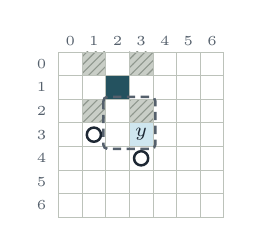
\begin{tikzpicture}[x=0.3cm,y=0.3cm,baseline=(current bounding box.north)]
\node[font=\tiny,text=inksoft] at (0.5,0.45) {0};
\node[font=\tiny,text=inksoft] at (1.5,0.45) {1};
\node[font=\tiny,text=inksoft] at (2.5,0.45) {2};
\node[font=\tiny,text=inksoft] at (3.5,0.45) {3};
\node[font=\tiny,text=inksoft] at (4.5,0.45) {4};
\node[font=\tiny,text=inksoft] at (5.5,0.45) {5};
\node[font=\tiny,text=inksoft] at (6.5,0.45) {6};
\node[font=\tiny,text=inksoft,anchor=east] at (-0.1,-0.5) {0};
\node[font=\tiny,text=inksoft,anchor=east] at (-0.1,-1.5) {1};
\node[font=\tiny,text=inksoft,anchor=east] at (-0.1,-2.5) {2};
\node[font=\tiny,text=inksoft,anchor=east] at (-0.1,-3.5) {3};
\node[font=\tiny,text=inksoft,anchor=east] at (-0.1,-4.5) {4};
\node[font=\tiny,text=inksoft,anchor=east] at (-0.1,-5.5) {5};
\node[font=\tiny,text=inksoft,anchor=east] at (-0.1,-6.5) {6};
\fill[blockedc] (1,0) rectangle (2,-1);
\fill[pattern=north east lines,pattern color=hatch] (1,0) rectangle (2,-1);
\fill[blockedc] (3,0) rectangle (4,-1);
\fill[pattern=north east lines,pattern color=hatch] (3,0) rectangle (4,-1);
\fill[chosen] (2,-1) rectangle (3,-2);
\fill[blockedc] (1,-2) rectangle (2,-3);
\fill[pattern=north east lines,pattern color=hatch] (1,-2) rectangle (2,-3);
\fill[blockedc] (3,-2) rectangle (4,-3);
\fill[pattern=north east lines,pattern color=hatch] (3,-2) rectangle (4,-3);
\fill[focustint] (3,-3) rectangle (4,-4);
\draw[gridc,line width=0.3pt,step=1] (0,-7) grid (7,0);
\draw[ink,line width=0.9pt] (1.5,-3.5) circle (0.3);
\draw[ink,line width=0.9pt] (3.5,-4.5) circle (0.3);
\draw[inksoft,line width=0.9pt,rounded corners=1.5pt,densely dashed] (1.9,-1.9) rectangle (4.1,-4.1);
\node[font=\scriptsize\bfseries,text=ink] at (3.5,-3.5) {$y$};
\end{tikzpicture} & 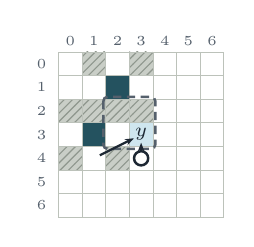
\begin{tikzpicture}[x=0.3cm,y=0.3cm,baseline=(current bounding box.north)]
\node[font=\tiny,text=inksoft] at (0.5,0.45) {0};
\node[font=\tiny,text=inksoft] at (1.5,0.45) {1};
\node[font=\tiny,text=inksoft] at (2.5,0.45) {2};
\node[font=\tiny,text=inksoft] at (3.5,0.45) {3};
\node[font=\tiny,text=inksoft] at (4.5,0.45) {4};
\node[font=\tiny,text=inksoft] at (5.5,0.45) {5};
\node[font=\tiny,text=inksoft] at (6.5,0.45) {6};
\node[font=\tiny,text=inksoft,anchor=east] at (-0.1,-0.5) {0};
\node[font=\tiny,text=inksoft,anchor=east] at (-0.1,-1.5) {1};
\node[font=\tiny,text=inksoft,anchor=east] at (-0.1,-2.5) {2};
\node[font=\tiny,text=inksoft,anchor=east] at (-0.1,-3.5) {3};
\node[font=\tiny,text=inksoft,anchor=east] at (-0.1,-4.5) {4};
\node[font=\tiny,text=inksoft,anchor=east] at (-0.1,-5.5) {5};
\node[font=\tiny,text=inksoft,anchor=east] at (-0.1,-6.5) {6};
\fill[blockedc] (1,0) rectangle (2,-1);
\fill[pattern=north east lines,pattern color=hatch] (1,0) rectangle (2,-1);
\fill[blockedc] (3,0) rectangle (4,-1);
\fill[pattern=north east lines,pattern color=hatch] (3,0) rectangle (4,-1);
\fill[chosen] (2,-1) rectangle (3,-2);
\fill[blockedc] (0,-2) rectangle (1,-3);
\fill[pattern=north east lines,pattern color=hatch] (0,-2) rectangle (1,-3);
\fill[blockedc] (1,-2) rectangle (2,-3);
\fill[pattern=north east lines,pattern color=hatch] (1,-2) rectangle (2,-3);
\fill[blockedc] (2,-2) rectangle (3,-3);
\fill[pattern=north east lines,pattern color=hatch] (2,-2) rectangle (3,-3);
\fill[blockedc] (3,-2) rectangle (4,-3);
\fill[pattern=north east lines,pattern color=hatch] (3,-2) rectangle (4,-3);
\fill[chosen] (1,-3) rectangle (2,-4);
\fill[focustint] (3,-3) rectangle (4,-4);
\fill[blockedc] (0,-4) rectangle (1,-5);
\fill[pattern=north east lines,pattern color=hatch] (0,-4) rectangle (1,-5);
\fill[blockedc] (2,-4) rectangle (3,-5);
\fill[pattern=north east lines,pattern color=hatch] (2,-4) rectangle (3,-5);
\draw[gridc,line width=0.3pt,step=1] (0,-7) grid (7,0);
\draw[ink,line width=0.9pt] (3.5,-4.5) circle (0.3);
\draw[inksoft,line width=0.9pt,rounded corners=1.5pt,densely dashed] (1.9,-1.9) rectangle (4.1,-4.1);
\draw[-{Stealth[length=3.2pt]},ink,line width=0.8pt,shorten <=0.084cm,shorten >=0.102cm] (1.5,-4.5) -- (3.5,-3.5);
\draw[-{Stealth[length=3.2pt]},ink,line width=0.8pt,shorten <=0.084cm,shorten >=0.102cm] (3.5,-4.5) -- (3.5,-3.5);
\node[font=\scriptsize\bfseries,text=ink] at (3.5,-3.5) {$y$};
\end{tikzpicture} & 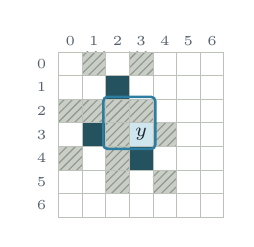
\begin{tikzpicture}[x=0.3cm,y=0.3cm,baseline=(current bounding box.north)]
\node[font=\tiny,text=inksoft] at (0.5,0.45) {0};
\node[font=\tiny,text=inksoft] at (1.5,0.45) {1};
\node[font=\tiny,text=inksoft] at (2.5,0.45) {2};
\node[font=\tiny,text=inksoft] at (3.5,0.45) {3};
\node[font=\tiny,text=inksoft] at (4.5,0.45) {4};
\node[font=\tiny,text=inksoft] at (5.5,0.45) {5};
\node[font=\tiny,text=inksoft] at (6.5,0.45) {6};
\node[font=\tiny,text=inksoft,anchor=east] at (-0.1,-0.5) {0};
\node[font=\tiny,text=inksoft,anchor=east] at (-0.1,-1.5) {1};
\node[font=\tiny,text=inksoft,anchor=east] at (-0.1,-2.5) {2};
\node[font=\tiny,text=inksoft,anchor=east] at (-0.1,-3.5) {3};
\node[font=\tiny,text=inksoft,anchor=east] at (-0.1,-4.5) {4};
\node[font=\tiny,text=inksoft,anchor=east] at (-0.1,-5.5) {5};
\node[font=\tiny,text=inksoft,anchor=east] at (-0.1,-6.5) {6};
\fill[blockedc] (1,0) rectangle (2,-1);
\fill[pattern=north east lines,pattern color=hatch] (1,0) rectangle (2,-1);
\fill[blockedc] (3,0) rectangle (4,-1);
\fill[pattern=north east lines,pattern color=hatch] (3,0) rectangle (4,-1);
\fill[chosen] (2,-1) rectangle (3,-2);
\fill[blockedc] (0,-2) rectangle (1,-3);
\fill[pattern=north east lines,pattern color=hatch] (0,-2) rectangle (1,-3);
\fill[blockedc] (1,-2) rectangle (2,-3);
\fill[pattern=north east lines,pattern color=hatch] (1,-2) rectangle (2,-3);
\fill[blockedc] (2,-2) rectangle (3,-3);
\fill[pattern=north east lines,pattern color=hatch] (2,-2) rectangle (3,-3);
\fill[blockedc] (3,-2) rectangle (4,-3);
\fill[pattern=north east lines,pattern color=hatch] (3,-2) rectangle (4,-3);
\fill[chosen] (1,-3) rectangle (2,-4);
\fill[blockedc] (2,-3) rectangle (3,-4);
\fill[pattern=north east lines,pattern color=hatch] (2,-3) rectangle (3,-4);
\fill[focustint] (3,-3) rectangle (4,-4);
\fill[blockedc] (4,-3) rectangle (5,-4);
\fill[pattern=north east lines,pattern color=hatch] (4,-3) rectangle (5,-4);
\fill[blockedc] (0,-4) rectangle (1,-5);
\fill[pattern=north east lines,pattern color=hatch] (0,-4) rectangle (1,-5);
\fill[blockedc] (2,-4) rectangle (3,-5);
\fill[pattern=north east lines,pattern color=hatch] (2,-4) rectangle (3,-5);
\fill[chosen] (3,-4) rectangle (4,-5);
\fill[blockedc] (2,-5) rectangle (3,-6);
\fill[pattern=north east lines,pattern color=hatch] (2,-5) rectangle (3,-6);
\fill[blockedc] (4,-5) rectangle (5,-6);
\fill[pattern=north east lines,pattern color=hatch] (4,-5) rectangle (5,-6);
\draw[gridc,line width=0.3pt,step=1] (0,-7) grid (7,0);
\draw[focus,line width=0.9pt,rounded corners=1.5pt] (1.9,-1.9) rectangle (4.1,-4.1);
\node[font=\scriptsize\bfseries,text=ink] at (3.5,-3.5) {$y$};
\end{tikzpicture}\\[4pt]
\footnotesize $\T{(1,2),(3,1),(4,3)}\to y$ & \footnotesize $\T{(3,1),(4,3)}\to y$ & \footnotesize $\T{(4,3)}\to y$ & \footnotesize $\T{\,}\to y$: forced\\
\footnotesize vacuum: a triple & \footnotesize (1,2) chosen: a pair & \footnotesize (3,1) chosen: a link & \footnotesize (4,3) chosen: a seat
\end{tabular}
\caption{One condition of $y=(3,3)$ collapsing. In the third frame a second term of $y$ gives the link $(4,1)\to y$ as well.}
\end{figure}

\onmap
\textbf{Seat rule:} a block with three corners blocked and one free: the free cell must be chosen. It acts on the present state, when the third corner gets blocked. Before that, the map shows only partly blocked blocks.

\interms
\begin{center}\small
\begin{tabular}{@{}lll@{}}
\toprule
size & name & meaning\\
\midrule
3 & vacuum term & three placements make $y$ a seat\\
2 & pair & two placements make $y$ a seat\\
1 & \textbf{link} $a\to y$ & choosing $a$ makes $y$ a seat: $a$ forces $y$\\
0 & forced & $y$ is a seat now (the seat rule)\\
\bottomrule
\end{tabular}
\end{center}
A link is a term collapsed to one member. It is the single-member case of the old pipeline's \code{forced\_by1}. \incode{}

%------------------------------------------------------------------
\section{Paths and aliasing}

\onmap
\begin{figure}[H]\centering
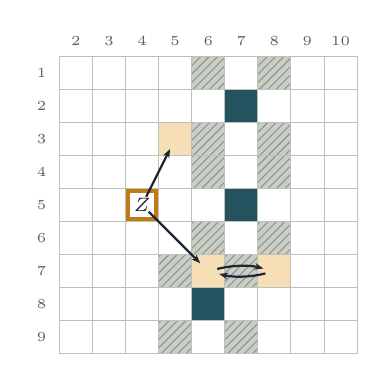
\begin{tikzpicture}[x=0.42cm,y=0.42cm,baseline=(current bounding box.north)]
\node[font=\tiny,text=inksoft] at (0.5,0.45) {2};
\node[font=\tiny,text=inksoft] at (1.5,0.45) {3};
\node[font=\tiny,text=inksoft] at (2.5,0.45) {4};
\node[font=\tiny,text=inksoft] at (3.5,0.45) {5};
\node[font=\tiny,text=inksoft] at (4.5,0.45) {6};
\node[font=\tiny,text=inksoft] at (5.5,0.45) {7};
\node[font=\tiny,text=inksoft] at (6.5,0.45) {8};
\node[font=\tiny,text=inksoft] at (7.5,0.45) {9};
\node[font=\tiny,text=inksoft] at (8.5,0.45) {10};
\node[font=\tiny,text=inksoft,anchor=east] at (-0.1,-0.5) {1};
\node[font=\tiny,text=inksoft,anchor=east] at (-0.1,-1.5) {2};
\node[font=\tiny,text=inksoft,anchor=east] at (-0.1,-2.5) {3};
\node[font=\tiny,text=inksoft,anchor=east] at (-0.1,-3.5) {4};
\node[font=\tiny,text=inksoft,anchor=east] at (-0.1,-4.5) {5};
\node[font=\tiny,text=inksoft,anchor=east] at (-0.1,-5.5) {6};
\node[font=\tiny,text=inksoft,anchor=east] at (-0.1,-6.5) {7};
\node[font=\tiny,text=inksoft,anchor=east] at (-0.1,-7.5) {8};
\node[font=\tiny,text=inksoft,anchor=east] at (-0.1,-8.5) {9};
\fill[blockedc] (4,0) rectangle (5,-1);
\fill[pattern=north east lines,pattern color=hatch] (4,0) rectangle (5,-1);
\fill[blockedc] (6,0) rectangle (7,-1);
\fill[pattern=north east lines,pattern color=hatch] (6,0) rectangle (7,-1);
\fill[chosen] (5,-1) rectangle (6,-2);
\fill[candtint] (3,-2) rectangle (4,-3);
\fill[blockedc] (4,-2) rectangle (5,-3);
\fill[pattern=north east lines,pattern color=hatch] (4,-2) rectangle (5,-3);
\fill[blockedc] (6,-2) rectangle (7,-3);
\fill[pattern=north east lines,pattern color=hatch] (6,-2) rectangle (7,-3);
\fill[blockedc] (4,-3) rectangle (5,-4);
\fill[pattern=north east lines,pattern color=hatch] (4,-3) rectangle (5,-4);
\fill[blockedc] (6,-3) rectangle (7,-4);
\fill[pattern=north east lines,pattern color=hatch] (6,-3) rectangle (7,-4);
\fill[chosen] (5,-4) rectangle (6,-5);
\fill[blockedc] (4,-5) rectangle (5,-6);
\fill[pattern=north east lines,pattern color=hatch] (4,-5) rectangle (5,-6);
\fill[blockedc] (6,-5) rectangle (7,-6);
\fill[pattern=north east lines,pattern color=hatch] (6,-5) rectangle (7,-6);
\fill[blockedc] (3,-6) rectangle (4,-7);
\fill[pattern=north east lines,pattern color=hatch] (3,-6) rectangle (4,-7);
\fill[candtint] (4,-6) rectangle (5,-7);
\fill[blockedc] (5,-6) rectangle (6,-7);
\fill[pattern=north east lines,pattern color=hatch] (5,-6) rectangle (6,-7);
\fill[candtint] (6,-6) rectangle (7,-7);
\fill[chosen] (4,-7) rectangle (5,-8);
\fill[blockedc] (3,-8) rectangle (4,-9);
\fill[pattern=north east lines,pattern color=hatch] (3,-8) rectangle (4,-9);
\fill[blockedc] (5,-8) rectangle (6,-9);
\fill[pattern=north east lines,pattern color=hatch] (5,-8) rectangle (6,-9);
\draw[gridc,line width=0.3pt,step=1] (0,-9) grid (9,0);
\draw[candc,line width=1.4pt] (2.07,-4.07) rectangle (2.93,-4.93);
\draw[-{Stealth[length=3.2pt]},ink,line width=0.8pt,shorten <=0.118cm,shorten >=0.143cm] (2.5,-4.5) -- (3.5,-2.5);
\draw[-{Stealth[length=3.2pt]},ink,line width=0.8pt,shorten <=0.118cm,shorten >=0.143cm] (2.5,-4.5) -- (4.5,-6.5);
\draw[-{Stealth[length=3.2pt]},ink,line width=0.8pt,shorten <=0.118cm,shorten >=0.143cm] (4.5,-6.5) to[bend left=14] (6.5,-6.5);
\draw[-{Stealth[length=3.2pt]},ink,line width=0.8pt,shorten <=0.118cm,shorten >=0.143cm] (6.5,-6.5) to[bend left=14] (4.5,-6.5);
\node[font=\scriptsize\bfseries,text=ink] at (2.5,-4.5) {$Z$};
\end{tikzpicture}\hspace{1cm}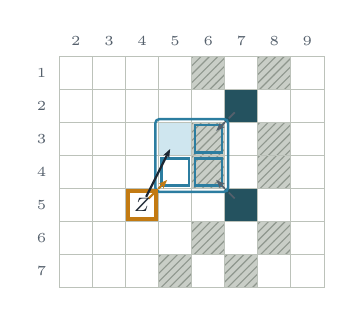
\begin{tikzpicture}[x=0.42cm,y=0.42cm,baseline=(current bounding box.north)]
\node[font=\tiny,text=inksoft] at (0.5,0.45) {2};
\node[font=\tiny,text=inksoft] at (1.5,0.45) {3};
\node[font=\tiny,text=inksoft] at (2.5,0.45) {4};
\node[font=\tiny,text=inksoft] at (3.5,0.45) {5};
\node[font=\tiny,text=inksoft] at (4.5,0.45) {6};
\node[font=\tiny,text=inksoft] at (5.5,0.45) {7};
\node[font=\tiny,text=inksoft] at (6.5,0.45) {8};
\node[font=\tiny,text=inksoft] at (7.5,0.45) {9};
\node[font=\tiny,text=inksoft,anchor=east] at (-0.1,-0.5) {1};
\node[font=\tiny,text=inksoft,anchor=east] at (-0.1,-1.5) {2};
\node[font=\tiny,text=inksoft,anchor=east] at (-0.1,-2.5) {3};
\node[font=\tiny,text=inksoft,anchor=east] at (-0.1,-3.5) {4};
\node[font=\tiny,text=inksoft,anchor=east] at (-0.1,-4.5) {5};
\node[font=\tiny,text=inksoft,anchor=east] at (-0.1,-5.5) {6};
\node[font=\tiny,text=inksoft,anchor=east] at (-0.1,-6.5) {7};
\fill[blockedc] (4,0) rectangle (5,-1);
\fill[pattern=north east lines,pattern color=hatch] (4,0) rectangle (5,-1);
\fill[blockedc] (6,0) rectangle (7,-1);
\fill[pattern=north east lines,pattern color=hatch] (6,0) rectangle (7,-1);
\fill[chosen] (5,-1) rectangle (6,-2);
\fill[focustint] (3,-2) rectangle (4,-3);
\fill[blockedc] (4,-2) rectangle (5,-3);
\fill[pattern=north east lines,pattern color=hatch] (4,-2) rectangle (5,-3);
\fill[blockedc] (6,-2) rectangle (7,-3);
\fill[pattern=north east lines,pattern color=hatch] (6,-2) rectangle (7,-3);
\fill[blockedc] (4,-3) rectangle (5,-4);
\fill[pattern=north east lines,pattern color=hatch] (4,-3) rectangle (5,-4);
\fill[blockedc] (6,-3) rectangle (7,-4);
\fill[pattern=north east lines,pattern color=hatch] (6,-3) rectangle (7,-4);
\fill[chosen] (5,-4) rectangle (6,-5);
\fill[blockedc] (4,-5) rectangle (5,-6);
\fill[pattern=north east lines,pattern color=hatch] (4,-5) rectangle (5,-6);
\fill[blockedc] (6,-5) rectangle (7,-6);
\fill[pattern=north east lines,pattern color=hatch] (6,-5) rectangle (7,-6);
\fill[blockedc] (3,-6) rectangle (4,-7);
\fill[pattern=north east lines,pattern color=hatch] (3,-6) rectangle (4,-7);
\fill[blockedc] (5,-6) rectangle (6,-7);
\fill[pattern=north east lines,pattern color=hatch] (5,-6) rectangle (6,-7);
\draw[gridc,line width=0.3pt,step=1] (0,-7) grid (8,0);
\draw[focus,line width=0.8pt] (4.09,-2.09) rectangle (4.91,-2.91);
\draw[focus,line width=0.8pt] (3.09,-3.09) rectangle (3.91,-3.91);
\draw[focus,line width=0.8pt] (4.09,-3.09) rectangle (4.91,-3.91);
\draw[focus,line width=0.9pt,rounded corners=1.5pt] (2.9,-1.9) rectangle (5.1,-4.1);
\draw[candc,line width=1.4pt] (2.07,-4.07) rectangle (2.93,-4.93);
\draw[-{Stealth[length=3.2pt]},inksoft,densely dashed,line width=0.6pt,shorten <=0.118cm,shorten >=0.143cm] (5.5,-1.5) -- (4.5,-2.5);
\draw[-{Stealth[length=3.2pt]},candc,densely dashed,line width=0.8pt,shorten <=0.118cm,shorten >=0.143cm] (2.5,-4.5) -- (3.5,-3.5);
\draw[-{Stealth[length=3.2pt]},inksoft,densely dashed,line width=0.6pt,shorten <=0.118cm,shorten >=0.143cm] (5.5,-4.5) -- (4.5,-3.5);
\draw[-{Stealth[length=3.2pt]},ink,line width=0.8pt,shorten <=0.118cm,shorten >=0.143cm] (2.5,-4.5) -- (3.5,-2.5);
\node[font=\scriptsize\bfseries,text=ink] at (2.5,-4.5) {$Z$};
\end{tikzpicture}
\caption{Left: chosen $(2,7),(5,7),(8,6)$. The links leaving $Z=(5,4)$: $Z\to(3,5)$, $Z\to(7,6)$, and $(7,6)\rightleftarrows(7,8)$, which force each other. Right: why $Z\to(3,5)$. In the block around pixel $(4,6)$, $(2,7)$ blocks $(3,6)$, $(5,7)$ blocks $(4,6)$, and $Z$ would block $(4,5)$.}
\end{figure}

\interms
\begin{figure}[H]\centering
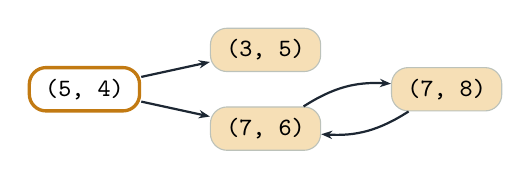
\begin{tikzpicture}
\node[draw=candc,line width=1.2pt,fill=white,rounded corners=6pt,minimum width=1.4cm,minimum height=0.55cm,font=\small\ttfamily] (n5_4) at (0,-0) {(5, 4)};
\node[draw=gridc,fill=candtint,rounded corners=6pt,minimum width=1.4cm,minimum height=0.55cm,font=\small\ttfamily] (n3_5) at (2.3,0.5) {(3, 5)};
\node[draw=gridc,fill=candtint,rounded corners=6pt,minimum width=1.4cm,minimum height=0.55cm,font=\small\ttfamily] (n7_6) at (2.3,-0.5) {(7, 6)};
\node[draw=gridc,fill=candtint,rounded corners=6pt,minimum width=1.4cm,minimum height=0.55cm,font=\small\ttfamily] (n7_8) at (4.6,-0) {(7, 8)};
\draw[-{Stealth[length=4pt]},ink,line width=0.8pt] (n5_4) to (n3_5);
\draw[-{Stealth[length=4pt]},ink,line width=0.8pt] (n5_4) to (n7_6);
\draw[-{Stealth[length=4pt]},ink,line width=0.8pt] (n7_6) to[bend left=18] (n7_8);
\draw[-{Stealth[length=4pt]},ink,line width=0.8pt] (n7_8) to[bend left=18] (n7_6);
\end{tikzpicture}
\caption{The same links as a graph, by distance from $Z$.}
\end{figure}
A \textbf{path} is a set of cells connected by links. The \textbf{aliases} of $Z$ are $Z$ and every cell reachable from $Z$ over links: $\mathrm{chosen}(Z)\Rightarrow\mathrm{chosen}(\text{each alias})$. Here: $\T{(5,4),(3,5),(7,6),(7,8)}$.

Aliasing is one-way. $(3,5)$ chosen does not force $Z$. A mutual link, like $(7,6)\rightleftarrows(7,8)$, makes two cells equivalent: either one chosen means both. A path can fan out ($Z$ has two links) and can contain cycles.

%------------------------------------------------------------------
\section{Candidate placement and its consequence}

\onmap
\begin{figure}[H]\centering
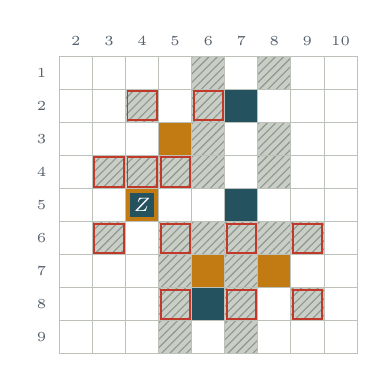
\begin{tikzpicture}[x=0.42cm,y=0.42cm,baseline=(current bounding box.north)]
\node[font=\tiny,text=inksoft] at (0.5,0.45) {2};
\node[font=\tiny,text=inksoft] at (1.5,0.45) {3};
\node[font=\tiny,text=inksoft] at (2.5,0.45) {4};
\node[font=\tiny,text=inksoft] at (3.5,0.45) {5};
\node[font=\tiny,text=inksoft] at (4.5,0.45) {6};
\node[font=\tiny,text=inksoft] at (5.5,0.45) {7};
\node[font=\tiny,text=inksoft] at (6.5,0.45) {8};
\node[font=\tiny,text=inksoft] at (7.5,0.45) {9};
\node[font=\tiny,text=inksoft] at (8.5,0.45) {10};
\node[font=\tiny,text=inksoft,anchor=east] at (-0.1,-0.5) {1};
\node[font=\tiny,text=inksoft,anchor=east] at (-0.1,-1.5) {2};
\node[font=\tiny,text=inksoft,anchor=east] at (-0.1,-2.5) {3};
\node[font=\tiny,text=inksoft,anchor=east] at (-0.1,-3.5) {4};
\node[font=\tiny,text=inksoft,anchor=east] at (-0.1,-4.5) {5};
\node[font=\tiny,text=inksoft,anchor=east] at (-0.1,-5.5) {6};
\node[font=\tiny,text=inksoft,anchor=east] at (-0.1,-6.5) {7};
\node[font=\tiny,text=inksoft,anchor=east] at (-0.1,-7.5) {8};
\node[font=\tiny,text=inksoft,anchor=east] at (-0.1,-8.5) {9};
\fill[blockedc] (4,0) rectangle (5,-1);
\fill[pattern=north east lines,pattern color=hatch] (4,0) rectangle (5,-1);
\fill[blockedc] (6,0) rectangle (7,-1);
\fill[pattern=north east lines,pattern color=hatch] (6,0) rectangle (7,-1);
\fill[blockedc] (2,-1) rectangle (3,-2);
\fill[pattern=north east lines,pattern color=hatch] (2,-1) rectangle (3,-2);
\fill[blockedc] (4,-1) rectangle (5,-2);
\fill[pattern=north east lines,pattern color=hatch] (4,-1) rectangle (5,-2);
\fill[chosen] (5,-1) rectangle (6,-2);
\fill[candc] (3,-2) rectangle (4,-3);
\fill[blockedc] (4,-2) rectangle (5,-3);
\fill[pattern=north east lines,pattern color=hatch] (4,-2) rectangle (5,-3);
\fill[blockedc] (6,-2) rectangle (7,-3);
\fill[pattern=north east lines,pattern color=hatch] (6,-2) rectangle (7,-3);
\fill[blockedc] (1,-3) rectangle (2,-4);
\fill[pattern=north east lines,pattern color=hatch] (1,-3) rectangle (2,-4);
\fill[blockedc] (2,-3) rectangle (3,-4);
\fill[pattern=north east lines,pattern color=hatch] (2,-3) rectangle (3,-4);
\fill[blockedc] (3,-3) rectangle (4,-4);
\fill[pattern=north east lines,pattern color=hatch] (3,-3) rectangle (4,-4);
\fill[blockedc] (4,-3) rectangle (5,-4);
\fill[pattern=north east lines,pattern color=hatch] (4,-3) rectangle (5,-4);
\fill[blockedc] (6,-3) rectangle (7,-4);
\fill[pattern=north east lines,pattern color=hatch] (6,-3) rectangle (7,-4);
\fill[chosen] (2,-4) rectangle (3,-5);
\fill[chosen] (5,-4) rectangle (6,-5);
\fill[blockedc] (1,-5) rectangle (2,-6);
\fill[pattern=north east lines,pattern color=hatch] (1,-5) rectangle (2,-6);
\fill[blockedc] (3,-5) rectangle (4,-6);
\fill[pattern=north east lines,pattern color=hatch] (3,-5) rectangle (4,-6);
\fill[blockedc] (4,-5) rectangle (5,-6);
\fill[pattern=north east lines,pattern color=hatch] (4,-5) rectangle (5,-6);
\fill[blockedc] (5,-5) rectangle (6,-6);
\fill[pattern=north east lines,pattern color=hatch] (5,-5) rectangle (6,-6);
\fill[blockedc] (6,-5) rectangle (7,-6);
\fill[pattern=north east lines,pattern color=hatch] (6,-5) rectangle (7,-6);
\fill[blockedc] (7,-5) rectangle (8,-6);
\fill[pattern=north east lines,pattern color=hatch] (7,-5) rectangle (8,-6);
\fill[blockedc] (3,-6) rectangle (4,-7);
\fill[pattern=north east lines,pattern color=hatch] (3,-6) rectangle (4,-7);
\fill[candc] (4,-6) rectangle (5,-7);
\fill[blockedc] (5,-6) rectangle (6,-7);
\fill[pattern=north east lines,pattern color=hatch] (5,-6) rectangle (6,-7);
\fill[candc] (6,-6) rectangle (7,-7);
\fill[blockedc] (3,-7) rectangle (4,-8);
\fill[pattern=north east lines,pattern color=hatch] (3,-7) rectangle (4,-8);
\fill[chosen] (4,-7) rectangle (5,-8);
\fill[blockedc] (5,-7) rectangle (6,-8);
\fill[pattern=north east lines,pattern color=hatch] (5,-7) rectangle (6,-8);
\fill[blockedc] (7,-7) rectangle (8,-8);
\fill[pattern=north east lines,pattern color=hatch] (7,-7) rectangle (8,-8);
\fill[blockedc] (3,-8) rectangle (4,-9);
\fill[pattern=north east lines,pattern color=hatch] (3,-8) rectangle (4,-9);
\fill[blockedc] (5,-8) rectangle (6,-9);
\fill[pattern=north east lines,pattern color=hatch] (5,-8) rectangle (6,-9);
\draw[gridc,line width=0.3pt,step=1] (0,-9) grid (9,0);
\draw[bad,line width=0.7pt] (2.06,-1.06) rectangle (2.94,-1.94);
\draw[bad,line width=0.7pt] (4.06,-1.06) rectangle (4.9399999999999995,-1.94);
\draw[bad,line width=0.7pt] (1.06,-3.06) rectangle (1.94,-3.94);
\draw[bad,line width=0.7pt] (2.06,-3.06) rectangle (2.94,-3.94);
\draw[bad,line width=0.7pt] (3.06,-3.06) rectangle (3.94,-3.94);
\draw[bad,line width=0.7pt] (1.06,-5.06) rectangle (1.94,-5.9399999999999995);
\draw[bad,line width=0.7pt] (3.06,-5.06) rectangle (3.94,-5.9399999999999995);
\draw[bad,line width=0.7pt] (5.06,-5.06) rectangle (5.9399999999999995,-5.9399999999999995);
\draw[bad,line width=0.7pt] (7.06,-5.06) rectangle (7.9399999999999995,-5.9399999999999995);
\draw[bad,line width=0.7pt] (3.06,-7.06) rectangle (3.94,-7.9399999999999995);
\draw[bad,line width=0.7pt] (5.06,-7.06) rectangle (5.9399999999999995,-7.9399999999999995);
\draw[bad,line width=0.7pt] (7.06,-7.06) rectangle (7.9399999999999995,-7.9399999999999995);
\draw[candc,line width=1.4pt] (2.07,-4.07) rectangle (2.93,-4.93);
\node[font=\scriptsize\bfseries,text=white] at (2.5,-4.5) {$Z$};
\end{tikzpicture}
\caption{$Z=(5,4)$ chosen and settled. Its aliases are chosen, and 12 cells are newly blocked (red outline).}
\end{figure}
A \textbf{candidate} is a free cell considered as a decision. In the pyramid it is a free cell of a placement tile, and each placement tile makes one decision. Its consequence: $Z$ and all its aliases are chosen, and their diagonal neighbours are blocked. Here, settling the map after choosing $Z$ places exactly the aliases $(3,5),(7,6),(7,8)$, nothing more.

\interms
For the terms, the consequence of a candidate is two lists: the alias set (members that drop out of terms) and the ring of cells they block (members whose terms die).

The map's links change: 32 links before, 37 after. The new ones are the candidate's consequences for others: cells that are now one placement away from a seat.

In general, settling can force more than the aliases: two aliases can together complete a pair term. That is the n-ary step, outside this document.

%------------------------------------------------------------------
\section{Blocked pairs}

\onmap
\begin{figure}[H]\centering
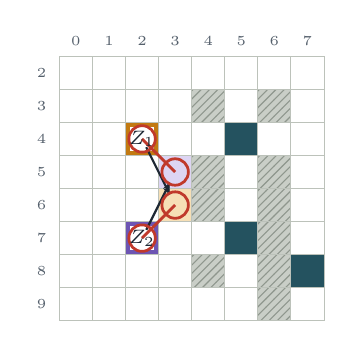
\begin{tikzpicture}[x=0.42cm,y=0.42cm,baseline=(current bounding box.north)]
\node[font=\tiny,text=inksoft] at (0.5,0.45) {0};
\node[font=\tiny,text=inksoft] at (1.5,0.45) {1};
\node[font=\tiny,text=inksoft] at (2.5,0.45) {2};
\node[font=\tiny,text=inksoft] at (3.5,0.45) {3};
\node[font=\tiny,text=inksoft] at (4.5,0.45) {4};
\node[font=\tiny,text=inksoft] at (5.5,0.45) {5};
\node[font=\tiny,text=inksoft] at (6.5,0.45) {6};
\node[font=\tiny,text=inksoft] at (7.5,0.45) {7};
\node[font=\tiny,text=inksoft,anchor=east] at (-0.1,-0.5) {2};
\node[font=\tiny,text=inksoft,anchor=east] at (-0.1,-1.5) {3};
\node[font=\tiny,text=inksoft,anchor=east] at (-0.1,-2.5) {4};
\node[font=\tiny,text=inksoft,anchor=east] at (-0.1,-3.5) {5};
\node[font=\tiny,text=inksoft,anchor=east] at (-0.1,-4.5) {6};
\node[font=\tiny,text=inksoft,anchor=east] at (-0.1,-5.5) {7};
\node[font=\tiny,text=inksoft,anchor=east] at (-0.1,-6.5) {8};
\node[font=\tiny,text=inksoft,anchor=east] at (-0.1,-7.5) {9};
\fill[blockedc] (4,-1) rectangle (5,-2);
\fill[pattern=north east lines,pattern color=hatch] (4,-1) rectangle (5,-2);
\fill[blockedc] (6,-1) rectangle (7,-2);
\fill[pattern=north east lines,pattern color=hatch] (6,-1) rectangle (7,-2);
\fill[chosen] (5,-2) rectangle (6,-3);
\fill[cand2tint] (3,-3) rectangle (4,-4);
\fill[blockedc] (4,-3) rectangle (5,-4);
\fill[pattern=north east lines,pattern color=hatch] (4,-3) rectangle (5,-4);
\fill[blockedc] (6,-3) rectangle (7,-4);
\fill[pattern=north east lines,pattern color=hatch] (6,-3) rectangle (7,-4);
\fill[candtint] (3,-4) rectangle (4,-5);
\fill[blockedc] (4,-4) rectangle (5,-5);
\fill[pattern=north east lines,pattern color=hatch] (4,-4) rectangle (5,-5);
\fill[blockedc] (6,-4) rectangle (7,-5);
\fill[pattern=north east lines,pattern color=hatch] (6,-4) rectangle (7,-5);
\fill[chosen] (5,-5) rectangle (6,-6);
\fill[blockedc] (6,-5) rectangle (7,-6);
\fill[pattern=north east lines,pattern color=hatch] (6,-5) rectangle (7,-6);
\fill[blockedc] (4,-6) rectangle (5,-7);
\fill[pattern=north east lines,pattern color=hatch] (4,-6) rectangle (5,-7);
\fill[blockedc] (6,-6) rectangle (7,-7);
\fill[pattern=north east lines,pattern color=hatch] (6,-6) rectangle (7,-7);
\fill[chosen] (7,-6) rectangle (8,-7);
\fill[blockedc] (6,-7) rectangle (7,-8);
\fill[pattern=north east lines,pattern color=hatch] (6,-7) rectangle (7,-8);
\draw[gridc,line width=0.3pt,step=1] (0,-8) grid (8,0);
\draw[candc,line width=1.4pt] (2.07,-2.07) rectangle (2.93,-2.93);
\draw[cand2c,line width=1.4pt] (2.07,-5.07) rectangle (2.93,-5.93);
\draw[-{Stealth[length=3.2pt]},ink,line width=0.8pt,shorten <=0.118cm,shorten >=0.143cm] (2.5,-2.5) -- (3.5,-4.5);
\draw[-{Stealth[length=3.2pt]},ink,line width=0.8pt,shorten <=0.118cm,shorten >=0.143cm] (2.5,-5.5) -- (3.5,-3.5);
\draw[bad,line width=1pt] (2.5,-2.5) -- (3.5,-3.5) (2.5,-2.5) circle (0.4) (3.5,-3.5) circle (0.4);
\draw[bad,line width=1pt] (3.5,-4.5) -- (2.5,-5.5) (3.5,-4.5) circle (0.4) (2.5,-5.5) circle (0.4);
\node[font=\scriptsize\bfseries,text=ink] at (2.5,-2.5) {$Z_1$};
\node[font=\scriptsize\bfseries,text=ink] at (2.5,-5.5) {$Z_2$};
\end{tikzpicture}\hspace{1cm}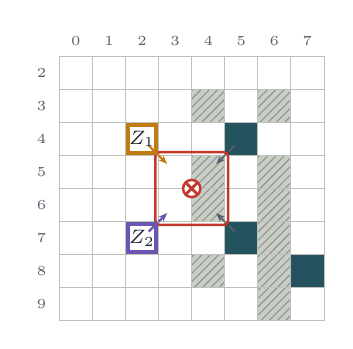
\begin{tikzpicture}[x=0.42cm,y=0.42cm,baseline=(current bounding box.north)]
\node[font=\tiny,text=inksoft] at (0.5,0.45) {0};
\node[font=\tiny,text=inksoft] at (1.5,0.45) {1};
\node[font=\tiny,text=inksoft] at (2.5,0.45) {2};
\node[font=\tiny,text=inksoft] at (3.5,0.45) {3};
\node[font=\tiny,text=inksoft] at (4.5,0.45) {4};
\node[font=\tiny,text=inksoft] at (5.5,0.45) {5};
\node[font=\tiny,text=inksoft] at (6.5,0.45) {6};
\node[font=\tiny,text=inksoft] at (7.5,0.45) {7};
\node[font=\tiny,text=inksoft,anchor=east] at (-0.1,-0.5) {2};
\node[font=\tiny,text=inksoft,anchor=east] at (-0.1,-1.5) {3};
\node[font=\tiny,text=inksoft,anchor=east] at (-0.1,-2.5) {4};
\node[font=\tiny,text=inksoft,anchor=east] at (-0.1,-3.5) {5};
\node[font=\tiny,text=inksoft,anchor=east] at (-0.1,-4.5) {6};
\node[font=\tiny,text=inksoft,anchor=east] at (-0.1,-5.5) {7};
\node[font=\tiny,text=inksoft,anchor=east] at (-0.1,-6.5) {8};
\node[font=\tiny,text=inksoft,anchor=east] at (-0.1,-7.5) {9};
\fill[blockedc] (4,-1) rectangle (5,-2);
\fill[pattern=north east lines,pattern color=hatch] (4,-1) rectangle (5,-2);
\fill[blockedc] (6,-1) rectangle (7,-2);
\fill[pattern=north east lines,pattern color=hatch] (6,-1) rectangle (7,-2);
\fill[chosen] (5,-2) rectangle (6,-3);
\fill[blockedc] (4,-3) rectangle (5,-4);
\fill[pattern=north east lines,pattern color=hatch] (4,-3) rectangle (5,-4);
\fill[blockedc] (6,-3) rectangle (7,-4);
\fill[pattern=north east lines,pattern color=hatch] (6,-3) rectangle (7,-4);
\fill[blockedc] (4,-4) rectangle (5,-5);
\fill[pattern=north east lines,pattern color=hatch] (4,-4) rectangle (5,-5);
\fill[blockedc] (6,-4) rectangle (7,-5);
\fill[pattern=north east lines,pattern color=hatch] (6,-4) rectangle (7,-5);
\fill[chosen] (5,-5) rectangle (6,-6);
\fill[blockedc] (6,-5) rectangle (7,-6);
\fill[pattern=north east lines,pattern color=hatch] (6,-5) rectangle (7,-6);
\fill[blockedc] (4,-6) rectangle (5,-7);
\fill[pattern=north east lines,pattern color=hatch] (4,-6) rectangle (5,-7);
\fill[blockedc] (6,-6) rectangle (7,-7);
\fill[pattern=north east lines,pattern color=hatch] (6,-6) rectangle (7,-7);
\fill[chosen] (7,-6) rectangle (8,-7);
\fill[blockedc] (6,-7) rectangle (7,-8);
\fill[pattern=north east lines,pattern color=hatch] (6,-7) rectangle (7,-8);
\draw[gridc,line width=0.3pt,step=1] (0,-8) grid (8,0);
\draw[bad,line width=0.9pt,rounded corners=1.5pt] (2.9,-2.9) rectangle (5.1,-5.1);
\draw[candc,line width=1.4pt] (2.07,-2.07) rectangle (2.93,-2.93);
\draw[cand2c,line width=1.4pt] (2.07,-5.07) rectangle (2.93,-5.93);
\filldraw[fill=white,draw=bad,line width=0.9pt] (4,-4) circle (0.26);
\draw[bad,line width=1pt] (3.83,-3.83) -- (4.17,-4.17) (3.83,-4.17) -- (4.17,-3.83);
\draw[-{Stealth[length=3.2pt]},candc,densely dashed,line width=0.8pt,shorten <=0.118cm,shorten >=0.143cm] (2.5,-2.5) -- (3.5,-3.5);
\draw[-{Stealth[length=3.2pt]},inksoft,densely dashed,line width=0.6pt,shorten <=0.118cm,shorten >=0.143cm] (5.5,-2.5) -- (4.5,-3.5);
\draw[-{Stealth[length=3.2pt]},inksoft,densely dashed,line width=0.6pt,shorten <=0.118cm,shorten >=0.143cm] (5.5,-5.5) -- (4.5,-4.5);
\draw[-{Stealth[length=3.2pt]},cand2c,densely dashed,line width=0.8pt,shorten <=0.118cm,shorten >=0.143cm] (2.5,-5.5) -- (3.5,-4.5);
\node[font=\scriptsize\bfseries,text=ink] at (2.5,-2.5) {$Z_1$};
\node[font=\scriptsize\bfseries,text=ink] at (2.5,-5.5) {$Z_2$};
\end{tikzpicture}
\caption{Left: chosen $(4,5),(7,5),(8,7)$. $Z_1=(4,2)$ forces $(6,3)$; $Z_2=(7,2)$ forces $(5,3)$. The red pairs are diagonal neighbours: $(4,2)/(5,3)$ and $(6,3)/(7,2)$. Right: both links come from one block, around pixel $(6,4)$. $(4,5)$ and $(7,5)$ block two of its corners. $Z_1$ blocks $(5,3)$, so $(6,3)$ must cover the pixel; $Z_2$ blocks $(6,3)$, so $(5,3)$ must. With both, all four corners are blocked: the hole of section 4.}
\end{figure}
Each candidate is fine alone. Together they cannot be chosen: they are a \textbf{blocked pair}, like two diagonal neighbours but at a distance.

\interms
No .conditions term says this today. The pair is recorded in the tiles' \code{.blocked} lists as $(Z_1,Z_2)$. \incode{} \code{Base.update\_blocked}.
\begin{algebra}
\cmt{defect term, block around pixel (6,4):}\\
$\T{(4,2),\,(4,5),\,(7,5),\,(7,2)} \;\longrightarrow\; \bot$\\
\cmt{(4,5), (7,5) chosen: they drop out}\\
$\T{(4,2),\,(7,2)} = \T{Z_1,Z_2} \;\longrightarrow\; \bot$
\end{algebra}
\proposed{} As a defect term, the blocked pair is that term reduced to two members, both candidates: $\neg(\mathrm{chosen}(Z_1)\wedge\mathrm{chosen}(Z_2))$. It has the same shape as the exclusion of two diagonal neighbours, which is the primitive rule behind ``blocked'' (section 2).

%------------------------------------------------------------------
\section{Refutation}

\onmap
\begin{figure}[H]\centering
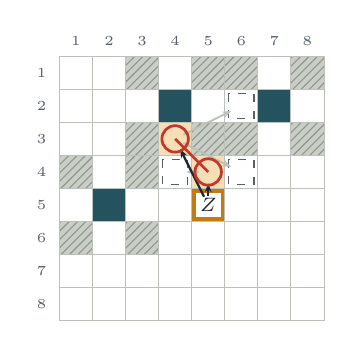
\begin{tikzpicture}[x=0.42cm,y=0.42cm,baseline=(current bounding box.north)]
\node[font=\tiny,text=inksoft] at (0.5,0.45) {1};
\node[font=\tiny,text=inksoft] at (1.5,0.45) {2};
\node[font=\tiny,text=inksoft] at (2.5,0.45) {3};
\node[font=\tiny,text=inksoft] at (3.5,0.45) {4};
\node[font=\tiny,text=inksoft] at (4.5,0.45) {5};
\node[font=\tiny,text=inksoft] at (5.5,0.45) {6};
\node[font=\tiny,text=inksoft] at (6.5,0.45) {7};
\node[font=\tiny,text=inksoft] at (7.5,0.45) {8};
\node[font=\tiny,text=inksoft,anchor=east] at (-0.1,-0.5) {1};
\node[font=\tiny,text=inksoft,anchor=east] at (-0.1,-1.5) {2};
\node[font=\tiny,text=inksoft,anchor=east] at (-0.1,-2.5) {3};
\node[font=\tiny,text=inksoft,anchor=east] at (-0.1,-3.5) {4};
\node[font=\tiny,text=inksoft,anchor=east] at (-0.1,-4.5) {5};
\node[font=\tiny,text=inksoft,anchor=east] at (-0.1,-5.5) {6};
\node[font=\tiny,text=inksoft,anchor=east] at (-0.1,-6.5) {7};
\node[font=\tiny,text=inksoft,anchor=east] at (-0.1,-7.5) {8};
\fill[blockedc] (2,0) rectangle (3,-1);
\fill[pattern=north east lines,pattern color=hatch] (2,0) rectangle (3,-1);
\fill[blockedc] (4,0) rectangle (5,-1);
\fill[pattern=north east lines,pattern color=hatch] (4,0) rectangle (5,-1);
\fill[blockedc] (5,0) rectangle (6,-1);
\fill[pattern=north east lines,pattern color=hatch] (5,0) rectangle (6,-1);
\fill[blockedc] (7,0) rectangle (8,-1);
\fill[pattern=north east lines,pattern color=hatch] (7,0) rectangle (8,-1);
\fill[chosen] (3,-1) rectangle (4,-2);
\fill[chosen] (6,-1) rectangle (7,-2);
\fill[blockedc] (2,-2) rectangle (3,-3);
\fill[pattern=north east lines,pattern color=hatch] (2,-2) rectangle (3,-3);
\fill[candtint] (3,-2) rectangle (4,-3);
\fill[blockedc] (4,-2) rectangle (5,-3);
\fill[pattern=north east lines,pattern color=hatch] (4,-2) rectangle (5,-3);
\fill[blockedc] (5,-2) rectangle (6,-3);
\fill[pattern=north east lines,pattern color=hatch] (5,-2) rectangle (6,-3);
\fill[blockedc] (7,-2) rectangle (8,-3);
\fill[pattern=north east lines,pattern color=hatch] (7,-2) rectangle (8,-3);
\fill[blockedc] (0,-3) rectangle (1,-4);
\fill[pattern=north east lines,pattern color=hatch] (0,-3) rectangle (1,-4);
\fill[blockedc] (2,-3) rectangle (3,-4);
\fill[pattern=north east lines,pattern color=hatch] (2,-3) rectangle (3,-4);
\fill[candtint] (4,-3) rectangle (5,-4);
\fill[chosen] (1,-4) rectangle (2,-5);
\fill[blockedc] (0,-5) rectangle (1,-6);
\fill[pattern=north east lines,pattern color=hatch] (0,-5) rectangle (1,-6);
\fill[blockedc] (2,-5) rectangle (3,-6);
\fill[pattern=north east lines,pattern color=hatch] (2,-5) rectangle (3,-6);
\draw[gridc,line width=0.3pt,step=1] (0,-8) grid (8,0);
\draw[inksoft,dashed,line width=0.5pt] (5.12,-1.12) rectangle (5.88,-1.88);
\draw[inksoft,dashed,line width=0.5pt] (3.12,-3.12) rectangle (3.88,-3.88);
\draw[inksoft,dashed,line width=0.5pt] (5.12,-3.12) rectangle (5.88,-3.88);
\draw[candc,line width=1.4pt] (4.07,-4.07) rectangle (4.93,-4.93);
\draw[-{Stealth[length=3.2pt]},gridc,line width=0.7pt,shorten <=0.118cm,shorten >=0.143cm] (3.5,-2.5) -- (5.5,-1.5);
\draw[-{Stealth[length=3.2pt]},gridc,line width=0.7pt,shorten <=0.118cm,shorten >=0.143cm] (3.5,-2.5) -- (5.5,-3.5);
\draw[-{Stealth[length=3.2pt]},gridc,line width=0.7pt,shorten <=0.118cm,shorten >=0.143cm] (4.5,-3.5) -- (3.5,-3.5);
\draw[-{Stealth[length=3.2pt]},ink,line width=0.8pt,shorten <=0.118cm,shorten >=0.143cm] (4.5,-4.5) -- (3.5,-2.5);
\draw[-{Stealth[length=3.2pt]},ink,line width=0.8pt,shorten <=0.118cm,shorten >=0.143cm] (4.5,-4.5) -- (4.5,-3.5);
\draw[bad,line width=1pt] (3.5,-2.5) -- (4.5,-3.5) (3.5,-2.5) circle (0.4) (4.5,-3.5) circle (0.4);
\node[font=\scriptsize\bfseries,text=ink] at (4.5,-4.5) {$Z$};
\end{tikzpicture}\hspace{1cm}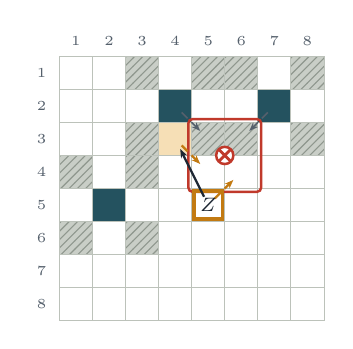
\begin{tikzpicture}[x=0.42cm,y=0.42cm,baseline=(current bounding box.north)]
\node[font=\tiny,text=inksoft] at (0.5,0.45) {1};
\node[font=\tiny,text=inksoft] at (1.5,0.45) {2};
\node[font=\tiny,text=inksoft] at (2.5,0.45) {3};
\node[font=\tiny,text=inksoft] at (3.5,0.45) {4};
\node[font=\tiny,text=inksoft] at (4.5,0.45) {5};
\node[font=\tiny,text=inksoft] at (5.5,0.45) {6};
\node[font=\tiny,text=inksoft] at (6.5,0.45) {7};
\node[font=\tiny,text=inksoft] at (7.5,0.45) {8};
\node[font=\tiny,text=inksoft,anchor=east] at (-0.1,-0.5) {1};
\node[font=\tiny,text=inksoft,anchor=east] at (-0.1,-1.5) {2};
\node[font=\tiny,text=inksoft,anchor=east] at (-0.1,-2.5) {3};
\node[font=\tiny,text=inksoft,anchor=east] at (-0.1,-3.5) {4};
\node[font=\tiny,text=inksoft,anchor=east] at (-0.1,-4.5) {5};
\node[font=\tiny,text=inksoft,anchor=east] at (-0.1,-5.5) {6};
\node[font=\tiny,text=inksoft,anchor=east] at (-0.1,-6.5) {7};
\node[font=\tiny,text=inksoft,anchor=east] at (-0.1,-7.5) {8};
\fill[blockedc] (2,0) rectangle (3,-1);
\fill[pattern=north east lines,pattern color=hatch] (2,0) rectangle (3,-1);
\fill[blockedc] (4,0) rectangle (5,-1);
\fill[pattern=north east lines,pattern color=hatch] (4,0) rectangle (5,-1);
\fill[blockedc] (5,0) rectangle (6,-1);
\fill[pattern=north east lines,pattern color=hatch] (5,0) rectangle (6,-1);
\fill[blockedc] (7,0) rectangle (8,-1);
\fill[pattern=north east lines,pattern color=hatch] (7,0) rectangle (8,-1);
\fill[chosen] (3,-1) rectangle (4,-2);
\fill[chosen] (6,-1) rectangle (7,-2);
\fill[blockedc] (2,-2) rectangle (3,-3);
\fill[pattern=north east lines,pattern color=hatch] (2,-2) rectangle (3,-3);
\fill[candtint] (3,-2) rectangle (4,-3);
\fill[blockedc] (4,-2) rectangle (5,-3);
\fill[pattern=north east lines,pattern color=hatch] (4,-2) rectangle (5,-3);
\fill[blockedc] (5,-2) rectangle (6,-3);
\fill[pattern=north east lines,pattern color=hatch] (5,-2) rectangle (6,-3);
\fill[blockedc] (7,-2) rectangle (8,-3);
\fill[pattern=north east lines,pattern color=hatch] (7,-2) rectangle (8,-3);
\fill[blockedc] (0,-3) rectangle (1,-4);
\fill[pattern=north east lines,pattern color=hatch] (0,-3) rectangle (1,-4);
\fill[blockedc] (2,-3) rectangle (3,-4);
\fill[pattern=north east lines,pattern color=hatch] (2,-3) rectangle (3,-4);
\fill[chosen] (1,-4) rectangle (2,-5);
\fill[blockedc] (0,-5) rectangle (1,-6);
\fill[pattern=north east lines,pattern color=hatch] (0,-5) rectangle (1,-6);
\fill[blockedc] (2,-5) rectangle (3,-6);
\fill[pattern=north east lines,pattern color=hatch] (2,-5) rectangle (3,-6);
\draw[gridc,line width=0.3pt,step=1] (0,-8) grid (8,0);
\draw[bad,line width=0.9pt,rounded corners=1.5pt] (3.9,-1.9) rectangle (6.1,-4.1);
\draw[candc,line width=1.4pt] (4.07,-4.07) rectangle (4.93,-4.93);
\filldraw[fill=white,draw=bad,line width=0.9pt] (5,-3) circle (0.26);
\draw[bad,line width=1pt] (4.83,-2.83) -- (5.17,-3.17) (4.83,-3.17) -- (5.17,-2.83);
\draw[-{Stealth[length=3.2pt]},inksoft,densely dashed,line width=0.6pt,shorten <=0.118cm,shorten >=0.143cm] (3.5,-1.5) -- (4.5,-2.5);
\draw[-{Stealth[length=3.2pt]},inksoft,densely dashed,line width=0.6pt,shorten <=0.118cm,shorten >=0.143cm] (6.5,-1.5) -- (5.5,-2.5);
\draw[-{Stealth[length=3.2pt]},candc,densely dashed,line width=0.8pt,shorten <=0.118cm,shorten >=0.143cm] (4.5,-4.5) -- (5.5,-3.5);
\draw[-{Stealth[length=3.2pt]},candc,densely dashed,line width=0.8pt,shorten <=0.118cm,shorten >=0.143cm] (3.5,-2.5) -- (4.5,-3.5);
\draw[-{Stealth[length=3.2pt]},ink,line width=0.8pt,shorten <=0.118cm,shorten >=0.143cm] (4.5,-4.5) -- (3.5,-2.5);
\node[font=\scriptsize\bfseries,text=ink] at (4.5,-4.5) {$Z$};
\end{tikzpicture}
\caption{Left: chosen $(2,4),(2,7),(5,2)$. $Z=(5,5)$ forces $(3,4)$ and $(4,5)$, which are diagonal neighbours (red). Dashed and grey: what the links go on to derive. It includes $(4,4)$ and $(4,6)$, $Z$'s own diagonal neighbours. Right: block around pixel $(4,6)$. $(2,4)$ and $(2,7)$ block two corners, $Z$ blocks $(4,6)$, and $(3,4)$, forced by $Z$, blocks $(4,5)$: the hole.}
\end{figure}
$Z$ forces two cells that block each other, so choosing $Z$ leads to a hole: $Z$ can never be chosen. Everything the links derive past this point assumes both cells chosen, and is worthless. \incode{} chains stop at their first contradiction (\code{Base.chain\_until\_contradiction}, and the n-ary step).

\interms
\begin{algebra}
$\T{(2,4),\,(2,7),\,(5,5),\,(3,4)} \;\longrightarrow\; \bot$\\
\cmt{(2,4), (2,7) chosen: they drop out}\\
$\T{(5,5),\,(3,4)} \;\longrightarrow\; \bot$\\
\cmt{(3,4) is an alias of $Z=(5,5)$}\\
$\T{Z} \;\longrightarrow\; \bot$: \ $Z$ is refuted
\end{algebra}
\proposed{} A \textbf{refutation} of $Z$ is a defect term all of whose remaining members are aliases of $Z$. The block around pixel $(4,4)$ gives a second one: $\T{(2,4),(5,2),Z,(4,5)}$.

\textbf{It is permanent.} More placements only shrink and kill terms. The links $Z\to(3,4)$ and $Z\to(4,5)$ were derived from cells that stay chosen. If one of $(3,4),(4,5)$ gets chosen from elsewhere, it blocks the other, which $Z$ still forces. If one gets blocked, $Z$ forces a blocked cell. Either way it is the hole again. A refuted $Z$ stays refuted in every later state.

\proposed{} So a refuted $Z$ is \textbf{blocked}: a defect term reduced to $\T{Z}$ has exactly the effect a chosen diagonal neighbour has. Every term with $Z$ as a member dies. This gives blocked cells two origins, both explained:
\begin{center}\small
\begin{tabular}{@{}lll@{}}
\toprule
origin & on the map & in .conditions\\
\midrule
exclusion & a chosen diagonal neighbour & primitive rule\\
refutation & choosing it leads to a hole & defect term collapsed to $\T{Z}$\\
\bottomrule
\end{tabular}
\end{center}

%------------------------------------------------------------------
\section*{Side by side}
\begin{center}\small
\begin{tabular}{@{}p{0.2\linewidth}p{0.36\linewidth}p{0.36\linewidth}@{}}
\toprule
notion & on the map & in .conditions\\
\midrule
cell & position of a 2$\times$2 square; covers 4 pixels & an id; a member of terms, the head of its own terms\\
condition & a block around $y$ with a blocker for each other corner & a term $\T{a,b,c}\to y$\\
chosen & square placed; diagonal neighbours blocked & member satisfied: drops out, term shrinks\\
blocked & never chosen; pixels may still be covered & member impossible: term dies; never named again\\
blocked 2$\times$2 block & a pixel no cell can cover: the hole & none today; \proposed{} defect term $\to\bot$\\
seat & 3 corners blocked, 1 free: the free one is forced & a term collapsed to size 0\\
link & one placement away from a seat & a term collapsed to size 1: $a\to y$\\
path, aliases & cells placed together with $Z$ & closure of $Z$ over links\\
candidate's consequence & aliases chosen, their diagonals blocked & alias set + blocked ring\\
blocked pair & $Z_1$ and $Z_2$ together leave a hole & \code{.blocked}; \proposed{} defect term reduced to $\T{Z_1,Z_2}$\\
refutation & $Z$ alone leaves a hole & \proposed{} defect term reduced to $\T{Z}$: $Z$ blocked\\
\bottomrule
\end{tabular}
\end{center}

\section*{Open questions}
\begin{enumerate}[leftmargin=*,itemsep=0.3em]
\item Where defect terms live (per block, i.e.\ per pixel), and how \code{compute\_conditions} reduces them: the same rules as for conditions, with $\bot$ in place of a cell.
\item Whether a refuted candidate is blocked for good rather than suspended for one pass. The permanence argument in section 9 holds as long as the real map and the rules stay fixed during a run.
\item Blocks outside the real map need no cover, so they get no defect terms. The margin's half- and quarter-cells need the same care as in \code{Base.restrict\_to\_real\_map}.
\item Blocked pairs: whether a defect term reduced to two candidates should be stored as a term or stay a \code{.blocked} entry.
\end{enumerate}

\end{document}
